\documentclass[tikz]{standalone}
\usetikzlibrary{shapes.geometric}
\usepackage{tikz}
\usepackage{standalone}
\begin{document}
	
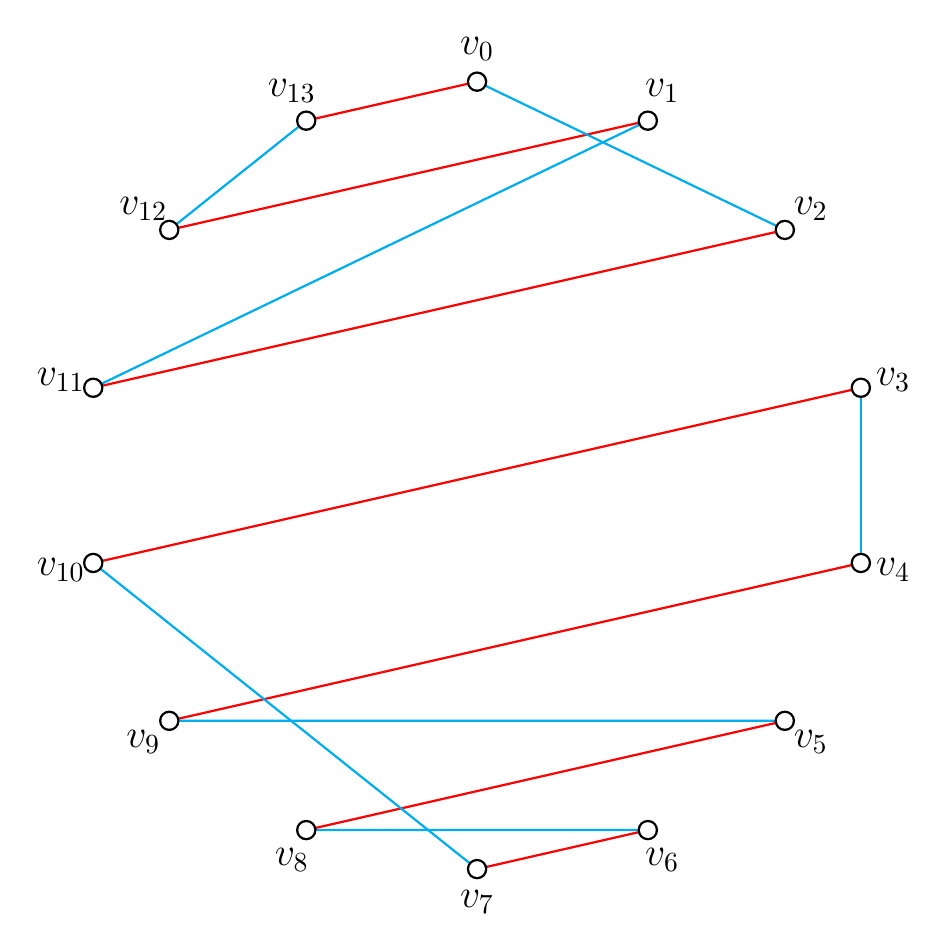
\begin{tikzpicture}
%Values of nodes:
% 0 = 1
% 1 = 1
% 2 = 2
% 3 = 2
% 4 = 3
% 5 = 3
% 6 = 4
% 7 = 4
% 8 = 4
% 9 = 5
% 10 = 5
% 11 = 6
% 12 = 7
% 13 = 7
% threshold tau = 7

\foreach \n in {0,...,13}
	\fill (90-\n*25.71428571:5cm) coordinate (v\n) circle [radius = 0.1]
		++(90-\n*25.71428571:12pt) node {\Large{$v_{\n}$}};
\foreach \m/\n in {0/13, 1/12, 2/11, 3/10, 4/9, 5/8, 6/7}
	\draw [thick, red] (v\n) -- (v\m);
\foreach \m/\n in {0/2, 1/11, 3/4, 5/9, 6/8, 7/10, 12/13}
	\draw [thick, cyan] (v\n) -- (v\m);
\foreach \n in {0,...,13}
	\fill (90-\n*25.71428571:5cm) coordinate (v\n) circle [radius = 0.13];
\foreach \n in {0,...,13}
	\fill [white] (90-\n*25.71428571:5cm) coordinate (v\n) circle [radius = 0.1];

\end{tikzpicture}
	
\end{document}